
\documentclass[journal=jacsat,manuscript=article]{achemso}


\usepackage{chemformula} 
\usepackage[T1]{fontenc} 
\usepackage{fixltx2e}
\usepackage{float}

\usepackage{caption}
\usepackage{subcaption}

\newcommand*\mycommand[1]{\texttt{\emph{#1}}}

\newcommand*{\figuretitle}[1]{%
    {\centering%   <--------  will only affect the title because of the grouping (by the
    \textbf{#1}%              braces before \centering and behind \medskip). If you remove
    \par\medskip}%            these braces the whole body of a {figure} env will be centered.
}

\captionsetup[figure]{labelformat=empty}

\author{Will Solow}
\email{whsolo22@colby.edu}
\author{Skye Rhomberg}
\email{sorhom22@colby.edu}
\author{Lindsey Madison}
\author{Eric Aaron}
\affiliation[Colby College]
{Department of Computer Science, Colby College, Waterville, ME}


\title{Investigating Zero-Point Energy in a Water Trimer with Diffusion Monte Carlo}


\begin{document}

\begin{abstract}
The Diffusion Monte Carlo (DMC) algorithm has been used to find solutions to the Schr\"dinger equation when no analytical solution is computable. The resulting wave function from the Sch\"odinger equation is of interest as it allows the physical properties of molecular systems to be better understood. We give a novel implementation of the DMC model in Python, highlighting the efficiency of NumPy’s vectorization techniques, in order to investigate the water molecule and water trimer systems. By running numerous trials of the implementation, we give necessary criteria to compute the resulting wave function of the Schr\"odinger equation and the Zero-Point Energy of the system. We give an overview of the difficulties encountered when instantiating a DMC simulation within a complicated molecular system and how this might extend to further work to more complex, heterogeneous molecular systems. By investigating the water molecule and water trimer, we provide a solid foundation for further work on utilizing the DMC model
\end{abstract}


\section{Introduction}

The Schrodinger\cite{Schrodinger1926} equation has been at the heart of physical chemistry given how the equation describes the wave function of a quantum system. Since its introduction, it has advanced the knowledge of quantum mechanics by allowing chemists to understand subatomic forces between atoms and molecules. However, solving the Schr\"odinger equation to determine the energies of a molecular system is difficult, and in practice can only be solved for a few simple molecular systems. The Schr\"odinger equation can explain many of the physical properties of water which are of great interest and have been studied extensively\cite{Goldman2004,Gillan2013}, yet many of the properties of water are still not fully understood.\cite{Liu1996}

The Diffusion Monte Carlo\cite{Anderson1975} (DMC) method allows for the Schr\"odinger wave function to be approximated for more complex systems using Monte Carlo methods given that the Schr\"odinger equation can only be solved analytically for a few specific molecular systems.\cite{Faber1996,Pang2014} For complex, many bodied systems\cite{Lee2019,Veil2001}, the DMC model is one of the few options as its computational complexity scales well with large input sizes. Even so, the DMC model remains a computationally hefty model for complex systems, even as the best option. 
	
As a complex molecular system, water is an ideal candidate to be studied using the DMC model\cite{Reynolds1982}. In fact, complex water structures, namely the hexamer, have been studied\cite{Babin2013,Severson1999}, albeit with simplifying assumptions. The DMC model is not without its limitations, however, and struggles with both population size of walkers\cite{Mallory2015} and time step\cite{Urimgar1993} (sampling) errors. 

To alleviate some of the computational load in a traditional DMC implementation, we presented a Python based implementation utilizing the NumPy library. NumPy provides tools to work efficiently through multidimensional matrices by splitting up the computational load amongst the cores of a computer’s processor to allow for simulations to be run faster. This method is not only faster, but allowed for the implementation of the DMC model to be generalized to a variety of homogeneous molecular systems. 

As such, the water molecule and the water trimer molecular system were investigated in order to find the wave function given by the Schr\"odinger equation and the Zero-Point Energy\cite{Gregory1996} (ZPE) of the system. Using this novel DMC implementation, we provide necessary simulation constants in order to accurately compute the wave function and ZPE within a desired variability. We also show how the selection of time step within the DMC model plays an important role in the convergence of both the walker population and the ZPE within the water molecule and water trimer systems. 
	
The specific aims of this project were to 1) employ a novel analytic implementation approach to study many-bodied molecular systems with the DMC model; 2) investigate the influence of different simulation constants on the ZPE for a single water molecule and water trimer; 3) determine the efficiency of the novel analytic implementation approach when compared with more traditional implementations. 


\section{Methods}

The methods for this project will be presented in the following sections: a description of the DMC model; the implementation of the model; and the validation steps that the researchers took to verify that the implementation was correct. 

\subsection{The Model}

 Professor Lindsey Madison provided pseudocode for the DMC model (see Appendix 1). The important constants in the model are dependent on the system being simulated. For this project which involved modeling a water molecule, the constants are: 1) the time step; this constant controls the distance over which the walkers can propagate during an iteration of the simulation loop; 2) the duration of the simulation; this constant is typically dependent on the time step in order to run the simulation for the same duration of real world time; 3) the number of copies of the same molecular system, also called the number of walkers in the simulation; 4) the masses of the molecules in the system; and 5) the equilibrium positions for the bond lengths and bond angles present in the system, typically calculated experimentally before use in the model. 

The time step dictates the distance over which each coordinate in each atom in each molecule in each walker moves from its starting position at the beginning of the iteration. Additionally, the time step also influences the acceptable range of the reference energy at each iteration of the simulation loop as well as the threshold for which an individual walker is replicated or deleted within the model. When the model is implemented correctly, the number of retained walkers should converge to the initial number of walkers.

The duration of the simulation is how many iterations of the simulation loop are run before the wave function and zero-point energy are calculated. Typically, a longer simulation gives more time for the molecular system to equilibrate. With smaller time steps, a longer simulation is necessary as equilibration takes many more iterations of the simulation loop given that the atoms are moving much shorter distances at each iteration towards equilibrium. 

The number of walkers determines the size of the walker list and can impact the range of an acceptable reference energy which, in turn, determines replication and deletion of walkers. Reference energy was determined as the average of the potential energy over all walkers plus a statistical constant which penalized populations of walkers larger than the initial value. The reference energy was used to calculate a 1000-step rolling average of the reference energy which converged to the ZPE. After equilibration, the average of the rolling average was used to calculate the ZPE of the simulation. We define this average as the ZPE\textsubscript{R} as it is the average of the rolling average of the reference energy. 

Typically, an equilibration phase was run with a duration based on the time step. Then, 10 to 20 production phases, which are repeated simulations of the DMC model, were run each of which calculates a ZPE. The average of the ZPE over these production phases we define as the ZPE\textsubscript{G} and is considered the computed ZPE of that trial. The ZPE\textsubscript{G}, along with the wave function, which was calculated based on the distribution of the bond lengths or bond angles in the molecular system, were considered the outputs of the DMC model. These outputs were then used as an approximation of the solution to Schrodinger’s equation.

\subsection{Implementation}

The implementation of the new model described above was broken down into three blocks of code. In the first block, the initial constants are described, and attention was only paid to the initial walker array. In the second block, the simulation loop was described and how it related to the DMC model. In the final block, the researchers gave an overview of the potential energy function. The implementation was broken down into these three blocks so that the code could be generalized to multiple systems in the future. The way the potential energy function was utilized in the simulation loop ensures that only the potential energy function needed to be changed when moving between molecular systems of study. 

To implement the new model described above, the researchers chose to store the initial walkers in a four-dimensional (4D) NumPy ndarray object. The researchers chose to use NumPy given that NumPy’s functions can operate quickly on multi-dimensional arrays. The 4D array had the following axes: the number of walkers by the number of molecules by the number of atoms in each molecule by the Cartesian coordinates (x, y, and z in 3D space). As a result, the researchers conjectured that the 4D array implementation could generalize to any system of homogeneous molecules. This data structure allowed the researchers to run trials on the single water molecule system and water trimer system without making any changes to the simulation loop. It should also be noted that this 4D array implementation allowed the code to be very readable. A 2D implementation was considered, with axes being the number of walkers by the coordinates of every atom in the system. However, the structure that the 4D array provides allowed for quick slicing and broadcasting of the array which made the code more easily understood.

In the simulation loop implementation, the researchers directly followed the pseudocode presented by the model. NumPy is able to operate on a large array of data simultaneously such that it was not necessary to use \textit{for loops} to access individual data points within the 4D array. The atoms in each walker were propagated by a pseudorandom number in the normal distribution of $\sqrt{\text{time step}/\text{atomic mass}}$. When studying the water molecule system, the researchers adopted the convention that the atom dimension of the 4D walker array would have the oxygen, hydrogen, hydrogen atoms in the same order each time. Given that each atom appeared in the same index in each walker in the 4D array, the NumPy tile function was used to broadcast the range of the normal distribution to each coordinate in the 4D array. This approach allowed for a one line propagation step within the simulation loop: 

\begin{figure}[H]
  \caption{Propagations of Walkers}
  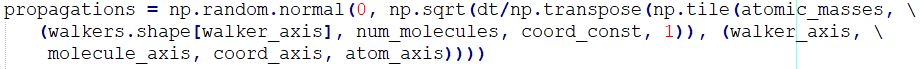
\includegraphics[width=\linewidth]{propagations.jpg}
\end{figure}

Another point of interest in the implementation of the simulation loop was the walker replication and deletion step. Based on the potential energy of each walker compared to the overall reference energy of the system and a random threshold number, the walker was selected to be either replicated or deleted from the 4D array. The index of each such walker was converted into a one-dimensional array of booleans with a \textit{True} value indicating that the walker should remain in the final walker array. NumPy arrays supported boolean indexing, so the implementation returned only the walkers that were not deleted and a copy of the walkers that were replicated.

The potential energy functions for the single water molecule and water trimer were perhaps the most interesting part of the simulation and were where the researchers could demonstrate the utility of NumPy. The researchers based the code on the potential energy functions provided by Professor Lindsey Madison. The researchers spent a significant amount of time understanding what the function did and brainstorming how to do those operations more efficiently in NumPy. The result was innovative yet unintuitive calculations that lent themselves to very efficient potential energy function calculations. For example, consider the line below within the water molecule intermolecular potential energy:

\begin{figure}[H]
  \caption{Intermolecular Distance Calculation}
  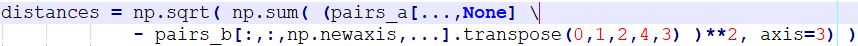
\includegraphics[width=\linewidth]{distances.jpg}
\end{figure}

The key insight was that the input to the potential energy function was a 4D array of walkers. To calculate the intermolecular potential energy, the function compared the distances between the atoms of every distinct pair of water molecules in the system. The researchers first used the NumPy array indexing to obtain arrays that have the distinct pairs (pair\_a and pair\_b). Then, considered the arrays that have the distinct pairs, notice that matrix multiplication behaves very similarly to distance calculation in that the corresponding elements are multiplied pointwise and then summed. However, pointwise multiplication was not exactly what was desired given that the distance between the two vectors was the variable of interest. NumPy performs matrix multiplication by broadcasting the array to a higher dimension, performing pointwise multiplication, and then summing along the extra axes resulting in a smaller array of the correct size. This was exactly what the code demonstrated, and the resulting array had the following dimensions: number of walkers by number of distinct pairs by number of atoms by number of atoms, where each datapoint was the distance between the atoms.

\subsection{Code Validation}

The next step was to validate the simulation loop separately from the potential energy function by using a CO harmonic oscillator given that the ZPE of the CO molecule has been calculated experimentally. If the calculated ZPE\textsubscript{R} of the system converged to the experimentally calculated ZPE, then the researchers could verify that the simulation loop was functioning correctly. The potential energy function of a harmonic oscillator system is $.5k(x-x_0)^2$, or the displacement of the oscillator from its equilibrium position. Without having to consider the accuracy of the potential energy function, the researchers were able to focus on validating the simulation loop. 
	
The simulation loop was validated in a variety of ways. The wave function, the main output of the DMC algorithm, is known and is given by the equation: $N\cdot \text{exp}[-(r^2)(\sqrt k\cdot mass)/2]$. When the implementation of the DMC algorithm is working correctly, the density histogram of the CO bond length will form a normal distribution that converges to the given wave function. Additionally, the ZPE of the CO molecule system was known to be .00494317, which had been calculated experimentally\cite{Madison2020}. The implementation of the DMC algorithm was considered correct if the 1000-step rolling average of the reference energy converged to .00494317 within the range of $1\cdot10^{-4}$\cite{Madison2020}. 
	
Given how NumPy was utilized in the implementation of the model, it was not self-evident that the replication and deletion of the walkers were mutually exclusive. The model would be ineffective if the same walker was both replicated and deleted in the same iteration of the simulation loop. To verify that this was not the case, auxiliary code was generated, and the replication and deletion step was tested using known unit values, or values where the expected outcome is predetermined. These values were useful as it was already known in advance which values would be replicated and deleted based on the way the test was run. Thus, the result of the replication and deletion steps were able to be compared to the expected outcome to verify that they were the same.

Finally, the propagation of the walkers was tested given that the NumPy tile function was utilized, which is not a traditional implementation. Again, the researchers turned to unit testing to verify that the code written was working correctly. Given that the propagation step chooses from a normal distribution based on the mass of the system, masses with drastically different magnitudes would yield very different results at different indices of the 4D array. As such, by printing an array of randomly generated propagations using masses with different magnitudes, the researchers were able to confirm that the correct index in the 4D array was being propagated within the correct magnitude. 

With the simulation loop validated, the researchers turned to the potential energy function in the single water molecule which calculated the intramolecular potential energy of the water moleculesystem. Our collaborator Dr. Lindsey Madison provided Python code that had already been validated as correct in corroboration with experimental results on the water molecule.\cite{Stillinger1975} The researchers’ goal was then to replicate the outputs of Dr. Madison’s code on different inputs. Once this was done, the intramolecular potential energy function was assumed to be correct. Given that the OH bond in a water molecule behaves much like a harmonic oscillator, the researchers were able to confirm that the convergence of the water molecule gave an OH bond length in the normal distribution given by the wave function of the corresponding harmonic oscillator. 

This process was repeated for the intermolecular potential energy in the water trimer. The researchers can confirm that the output of the code matches previous versions of the code up to the 18th decimal place. However, the ZPE convergence behaviour of the water trimer is an open research question. It is expected that the oxygen atoms in the trimer form a equiangular triangle\cite{Madison2020}, so a normal distribution of oxygen angles centered at 60 degrees would be expected. However, future work will determine what simulation constants are sufficient to observe this behaviour given the stochastic nature of the DMC algorithm.

\section{Simulations}

To investigate the ZPE of the water molecule and water trimer, the researchers employed the following strategy. Using the simulation loop, an equilibrated array of walkers was created and stored for later use. At the beginning of each trial, this equilibrated array of walkers was put through another equilibration phase with a duration based on the time step. A system in equilibrium will not deviate far from equilibrium; it will only move around slightly. This process served to randomize the start of our production phases to ensure that the data that was generated were from a random distribution of possible molecular system configurations. There are other methods to equilibrate a system such as choosing a number within a uniform distribution. This method was performed for the water molecule, and coordinates were chosen uniformly within the range [0,1). This was possible to perform with the water trimer as well\cite{Roinou2020}, however the researchers chose to work from a previously equilibrated array of walkers as the former method led to a large increase in the walker population before returning to the initial value, adding to the trial run time. 

The researchers ran trials with timesteps of [10,5,1,0.5,0.1] with initial walker populations of [1000,5000,10000] over 10 or 20 production phases. In each trial, a walker array was equilibrated and then put through a series of production phases to determine the ZPE\textsubscript{G}. Over the 10 trials for each of these variables, an average of the ZPE\textsubscript{G} was calculated, labeled the ZPE\textsubscript{T}. Calculating the ZPE\textsubscript{T} in this case was not equivalent to calculating a ZPE\textsubscript{G} with 100 production phases. This was due to the fact that each ZPE\textsubscript{G} was calculated from one initial equilibration phase which the production phases are run from. Furthermore, the researchers were interested in the standard deviation of the ZPE\textsubscript{G} calculated as well, so by computing the ZPE\textsubscript{G} over the 10 trials, the researchers could quantify how the simulation constants affected both the variability in the ZPE\textsubscript{G} as well as its computed value.

Using the existing implementation of the intramolecular potential energy function given by Professor Lindsey Madison, and the NumPy 4D array implementation described above, simulations were run and similar ZPE\textsubscript{R} values were obtained, further confirming the validation of the newer model. The run time for the simulations using both implementations of the potential energy function were recorded and compared by an empirical analysis over varying populations of walkers and simulation iterations. The time step was kept constant at 0.1, given that such a time step gave a walker population convergent to 99.99\% of initial value.

\section{Results}

By decreasing the time step or by increasing the number of walkers, the ZPE\textsubscript{T} (the average of the ZPE\textsubscript{G} over 10 trials) increased between time steps of 10 to 1.0 and then plateaued at time steps lower than 1.0 (Figure 1A). However, note that at a time step of 10, the ZPE\textsubscript{T} was noticeably lower than the ZPE\textsubscript{T} produced by smaller timesteps. Until recently, with the exploration of the water molecule system, a time step of 10 was considered sufficiently small to produce accurate results but this was not consistent with our results. In contrast, at the smaller time steps (e.g., 0.1 and 0.5), the ZPE\textsubscript{T} stayed constant, implying that it was in a desirable range. This result supported our findings that smaller time steps should be used in the modelling of more complicated systems. 

\begin{figure}
\centering
\figuretitle{Effects of Simulation Constants on Zero-Point Energy and Variability}
\begin{subfigure}{.5\textwidth}
  \centering
  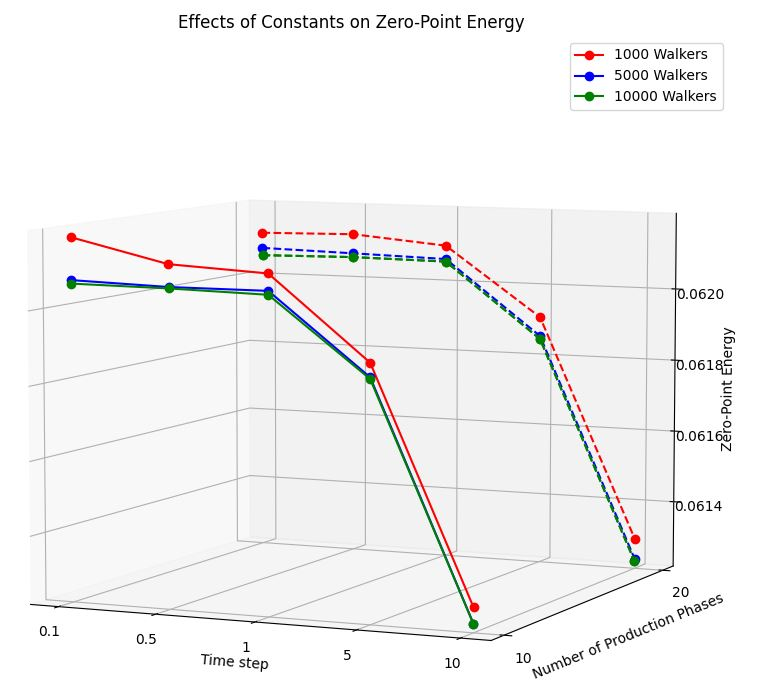
\includegraphics[width=\linewidth]{fig_1A.jpg}
\end{subfigure}%
\begin{subfigure}{.5\textwidth}
  \centering
  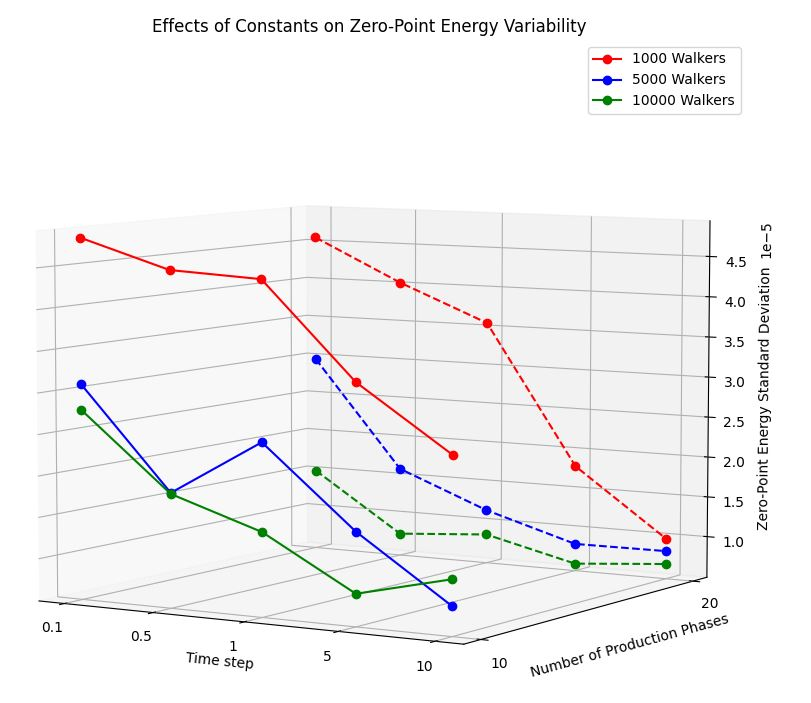
\includegraphics[width=\linewidth]{fig_1B}
\end{subfigure}
\caption{Figure 1A: The Zero Point Energy (ZPE\textsubscript{T} plateaus below a time step of 1.0. Increasing the walkers above 5000 or increasing the number of production phases does not alter the ZPE\textsubscript{T}\\ 
Figure 1B: The standard deviation of the Zero Point Energy}
\end{figure}

In addition to the calculated ZPE\textsubscript{T} of the system, the standard deviation of the ZPE\textsubscript{G} for each time step and walker population was investigated. While the overall average (the ZPE\textsubscript{T}) was important, a small variance was also desirable as it demonstrated that the simulation produced similar results consistently. In Figure 1B, we showed how the standard deviation consistently decreased with both an increase in walker population and an increase in the number of production phases over which the ZPE\textsubscript{G} was calculated. However, of interest was that a larger time step drastically decreased the standard deviation of the ZPE\textsubscript{G}, which will be highlighted in the Discussion. 

\begin{figure}[H]
  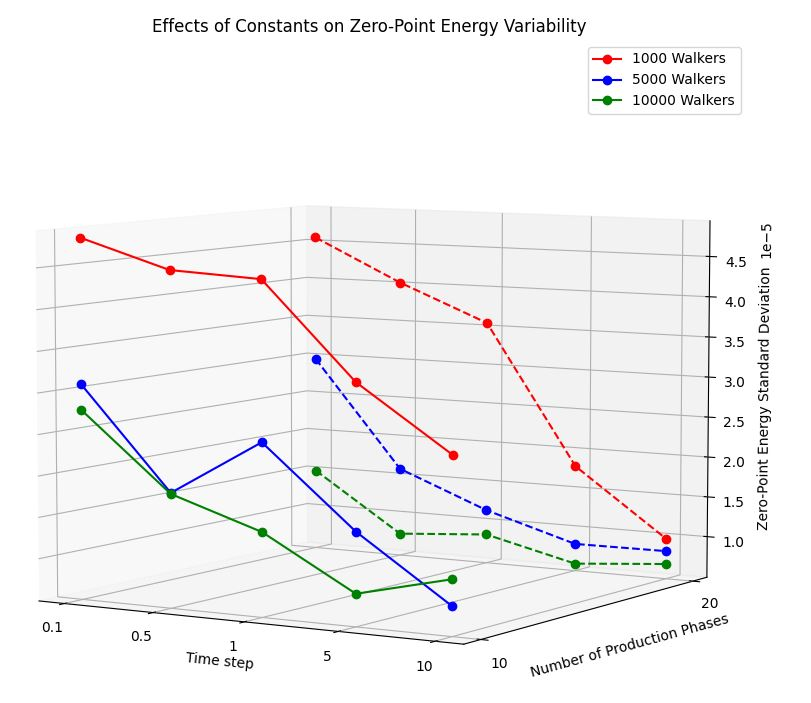
\includegraphics[width=\linewidth]{fig_1B.jpg}
  \caption{Figure 1B}
  \label{fig:}
\end{figure}

In Figure 3A, we show the equilibrium walker population at the end of the production phase compared to the ZPE\textsubscript{G} calculated. A retained walker population of 100\% is ideal. The percent of walkers retained at the end of the simulation remained virtually unchanged with more production phases or more walkers; thus, Figure 2 only shows the data for 10000 walkers over 20 production phases. We concluded that a decrease in time step is directly correlated to an increase in the remaining walker population. Furthermore, the connection between walker population and ZPE\textsubscript{T} was illuminated in that fewer remaining walkers resulted in a smaller ZPE\textsubscript{T}, which was assumed to be more inaccurate when modelling the water molecule system. 

\begin{figure}[H]
  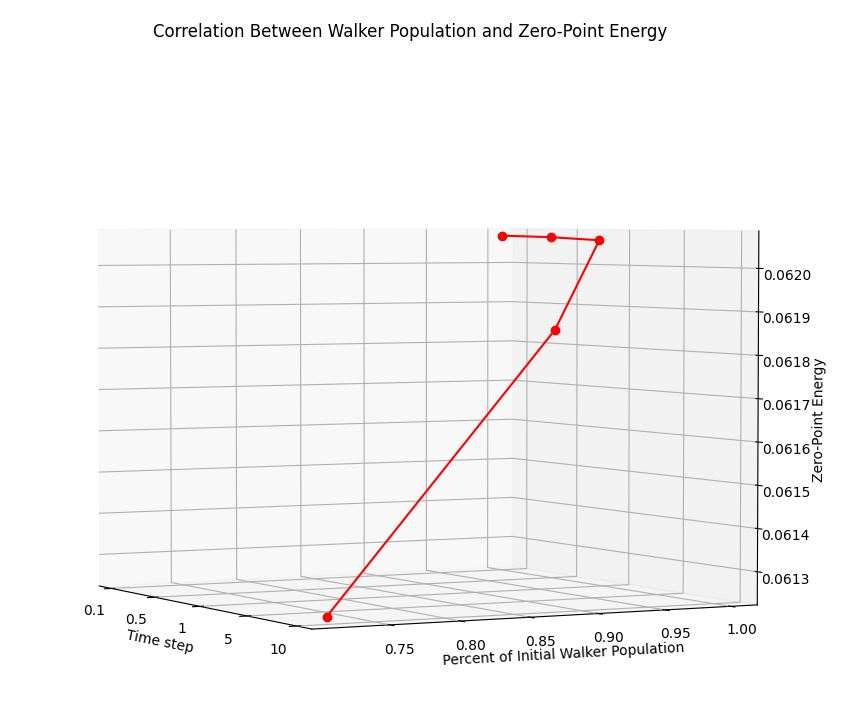
\includegraphics[width=\linewidth]{fig_2.jpg}
  \caption{Figure 2}
  \label{fig:}
\end{figure}

In contrast, Figure 3 demonstrated that a smaller time step was correlated with a larger standard deviation. That said, a smaller time step gave a presumably more accurate ZPE\textsubscript{T}, and combined with a convergence of the ZPE\textsubscript{T} calculated after a time step of 1.0, we saw that such a smaller time step was a necessary condition for calculating the correct ZPE\textsubscript{T} value. Note that the standard deviation was still minimal with a small time step, and can be lowered by adding production phases or more walkers. Typically, a smaller time step would be associated with more accurate results and a smaller variance. Here we saw more accurate results in a higher ZPE\textsubscript{T}, but also see the variance increase. Reasons for this finding was highlighted in the Discussion section.

\begin{figure}[H]
  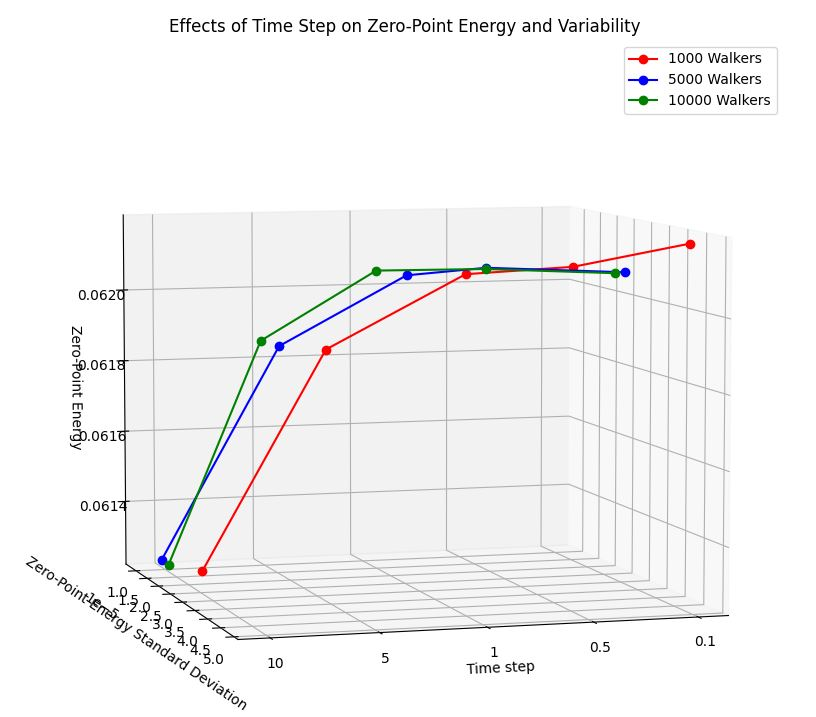
\includegraphics[width=\linewidth]{fig_3.jpg}
  \caption{Figure 3}
  \label{fig:}
\end{figure}

By incorporating the novel analytic model, the run times improved from 32 to 45 times faster than the existing model for simulating a single water model. Table 1 shows the rate at which the Solow-Rhomberg intramolecular potential energy function improved over the Madison intramolecular potential energy function. All simulations were run using the simulation loop generated by the researchers. Ten trials were run for each walker value and simulation duration to obtain an average. Notably, for 10000 walkers over 10000 time steps, the Solow-Rhomberg potential energy function yielded an average run time of 66 seconds while the Madison potential energy function yielded an average run time of 2644 seconds, giving an improvement rate of 39.75.

The efficiencies gained by using NumPy have implications for expanding the model to a water timer. To obtain a meaningful result from the water trimer takes around an hour. We would expect that more complicated molecular systems take longer given the extra computations required in the potential energy function and given that there are more atoms present in the system. As such, this run time improvement with the Solow-Rhomberg potential energy function only becomes more meaningful.

\section{Discussion}

Based on our results, we demonstrated that a time step of at most 1.0 is necessary to properly collect ZPE\textsubscript{G} data on the water molecule. We also demonstrated that both 10 and 20 production phases produced the same ZPE\textsubscript{G}; however, 20 production phases also lowered the standard deviation among the 10 ZPE\textsubscript{G} values that were calculated. More walkers lowered the standard deviation as well and impacted the ZPE\textsubscript{G} calculated when the initial walker population was less than 5000. Finally, we saw how the remaining walker population impacted the ZPE\textsubscript{G} and how it corresponded to the time step. All of this points to the fact that a smaller time step was better when modelling more complicated molecular systems. 

The importance of selecting the correct time step cannot be understated. With a smaller timestep the ZPE\textsubscript{G} calculated was more accurate. Moreover, the aim of the DMC algorithm was also to compute the wave function, or the normal distribution curve that the Schr\"odinger equation gives. With a larger timestep, the walker population was not convergent to its initial value. Thus with fewer retained walkers, the density histogram created did not converge to a normal curve. As a result, the wave function could not be calculated with a non-convergent walker population, which results from an incorrectly chosen time step. It should also be noted that a larger walker population gave rise to a histogram that converges closer to a normal curve. This was due to the fact that a larger sample size is more accommodating for small irregularities in the population, and therefore has a smoother density histogram. 

Our results demonstrated that a smaller time step led to a larger standard deviation in the ZPE\textsubscript{G} calculated. At first, this finding appears counterintuitive. However, in the simulation loop, the walkers were propagated in a normal distribution in the range of $\sqrt{\text{time step}/\text{mass}}$. A smaller time step meant that each atom in each walker could only move a smaller distance in each iteration of the simulation loop; this fact supports why the number of iterations needed to be normalized to the time step. In a complex molecular system like the water molecule, the length of both OH bonds and the HOH bond angle are enforced. With a larger time step, more motion occured at each iteration. Thus, it became easier for the walker to move outside an acceptable range from the reference energy, resulting in its deletion from the array. 

The allowance of extra motion was exactly what we saw with a larger time step in that enough walkers always moved out of an acceptable range at each iteration, resulting in a walker population that did not converge to the initial population. With regard to the standard deviation, we saw that with a larger time step, the range over which walkers were likely to move is increased, allowing a larger portion of the walkers to move outside an acceptable range at each step. When the walkers are deleted, they no longer contribute to the reference energy, resulting in a lower standard deviation because the walkers remaining were more identical to in their atom configuration to each other. In contrast, with a smaller time step less motion occured at each iteration. As a result, the walkers were able to move to the edge of an acceptable reference energy value without being deleted from the walker array given that they could move in small increments towards a non-valid atom configuration. As such, a smaller time step actually created more variance in the system, which was what we would expect as we got closer to simulating continuous time within a molecular system. 

As mentioned in the modelling section, our implementation of the DMC algorithm heavily utilized the NumPy library. NumPy’s vectorization techniques with matrices allowed the computations to be divided and thus computed efficiently among the cores of the computer. Different hardware architectures allow for more compatibility with vectorization techniques, but even on an older laptop, we still saw a noticeable decrease in run time on the order of 40 times faster than a more traditional DMC implementation. At the core of NumPy, however, the implementation still had to loop over every value within the 4D array. This explains why the implementation was a constant time improvement, and not a linear time improvement or better. Ultimately, we did not do anything meaningfully different in the computation in the simulation loop, but we did the same process much faster. Even so, an improvement of 40 times should not be underestimated as it was the difference between hours and days when running lengthy trials, particularly when more walkers or production phases were added.

\subsection{Limitations}

Today, some DMC implementations incorporate importance sampling\cite{Vihola2020} which is a strategy used to estimate the properties of a distribution while having only a sample at hand. As previously stated, the goal of the DMC algorithm waas to approximate the wave function of the Schr\"odinger equation. With only samples at hand, those samples being the number of walkers, importance sampling allows for the wave function to be approximated more accurately\cite{Bulik2018} given that the computational complexity of the algorithm limits the number of walkers on which trials can realistically be run. Future work may include adding importance-sampling techniques to our implementation. 

Time is always a limiting factor in computational sciences. Given that it is necessary to standardize the number of iterations in a simulation to the time step, running trials on smaller time steps takes drastically more time. Time permitting, we would have been interested in quantifying the behaviour of the ZPE\textsubscript{G} with time steps of .05 and .01 as well. Additionally, it would have been interesting to see the decrease in standard deviation continued if 30 or 50 production phases were used. Finally, we could have explored the trend in the ZPE\textsubscript{G} to determine if it remained unchanged after 10000 walkers. Running trials with 15000 and 20000 walkers should have been sufficient to confirm these conjectures.

\subsection{Future Work}

Moving forward, we hope to continue our investigations of the water trimer molecular system. We have strong data to support the necessary conditions for convergence of the ZPE\textsubscript{G} calculated based on the time step and walker populations. That said, we saw that the density histogram of the oxygen angles did not always converge to an expected normal distribution. Other convergence conditions also needed to be explored which involved the positions of the hydrogen atoms in one water molecule with respect to the oxygen atoms in the other two water molecules. If we can confirm that conditions are met, then, along with the ZPE\textsubscript{G} calculated, we will be able to determine with confidence that we have determined the ZPE\textsubscript{G} of the water trimer. 

Following the water trimer validation, we then hope to investigate clathrate hydrates\cite{Englezos1993}, also known as water cages. Clathrate hydrates present the unique challenge in that they are a system of heterogeneous molecules, unlike the systems that have been studied to date. The large advantage of NumPy is that it is very efficient for rectangular matrices. This advantage of rectangular matrices may be lost if we try to simulate clathrate hydrates in the same way as the water trimer system given that some entries of the 4D array would be empty because each molecule in the system does not have the same number of atoms. It is possible that we could avoid this problem by using NumPy’s masking feature or creating our own data type, but this remains to be investigated. 

Furthermore, the potential energy function for a clathrate hydrate molecule is likely much more complicated than a water trimer system. As such, we would expect the computational complexity of the system to be much greater. As a final obstacle, equilibration of the system becomes extraordinarily difficult. We have already seen that it is hard to equilibrate a water trimer from random values, given the magnitude of the randomness introduced into the system. Thus, by the same logic, it follows that a clathrate hydrate system would be equally challenging to obtain an equilibrium configuration on which to run simulations.

\section{Conclusion}

The DMC algorithm remains at the forefront of computational chemistry research given its ability to provide an approximation of a solution to the Shrodinger equation. Our work furthers the knowledge of the DMC algorithm by giving a unique and more efficient implementation leveraging NumPy. With this implementation, we investigated the water molecule and water trimer to show the influence of different simulation constants on the ZPE for a single water molecule. Our findings point to the necessary criteria needed to obtain accurate data from the simulation. 


%%%%%%%%%%%%%%%%%%%%%%%%%%%%%%%%%%%%%%%%%%%%%%%%%%%%%%%%%%%%%%%%%%%%%%
%%% The appropriate \bibliography command should be placed here.
%%% Notice that the class file automatically sets \bibliographystyle
%%% and also names the section correctly.
%%%%%%%%%%%%%%%%%%%%%%%%%%%%%%%%%%%%%%%%%%%%%%%%%%%%%%%%%%%%%%%%%%%%%%
\bibliography{rs_bib}

\end{document}
